%BAB_2 LAPORAN KP
\chapter{LANDASAN TEORI}

\section{Gambaran Umum Robot Lengan}

Robot adalah adalah sebuah alat yang terdiri dari gabungan mekanik dan elektronik yang dapat melakukan tugas fisik, baik menggunakan pengawasan dan kendali manusia maupun secara otomatis. Robot dapat melakukan suatu tugas secara berulang tanpa merasa lelah sehingga robot banyak digunakan dalam dunia industri khususnya pada bidang produksi. Salah satu jenis robot yang sering dalam bidang produksi adalah sistem lengan robot.

Robot lengan adalah robot yang memiliki bentuk fisik seperti halnya lengan pada manusia dan memiliki derajat kebebasan (degre of freedom) tertentu bergantung pada jumlah sendi yang digunakan. Dengan begitu robot lengan terdiri dari beberapa jenis. Robot lengan pada bidang industri biasa digunakan sebagai actuator untuk mengambil dan meletakkan suatu objek secara terus menerus.
	

Pada umumnya struktur robot lengan terdiri dari beberapa bagian.  Bagian utama adalah struktur mekanik (manipulator) yang merupakan susunan kerangka yang tidak dapat digerakkan (rigid) dan lengan (link) yang satu sama lain terhubung oleh sendi (joint). Dengan adanya joint yang menghubungkan dua link menjadi satu kesatuan sehingga joint membentuk satu derajat kebebasan. Jika diibaratkan dengan tubuh manusia, link adalah tulang sedangkan joint adalah sendi-sendinya. Joint memiliki dua pergerakan, yaitu pergerakan revolute joint (gerak berputar) dan prismatic joint (gerak bergeser) seperti yang ditunjukkan oleh Gambar 2.1

	\begin{figure}[H]
	\centering
	\includegraphics[width=10cm]{gambar/joint.png}
	\caption{Jenis-Jenis \emph Joint}
\end{figure}

Pada ujung pangkal lengan, robot lengan umumnya menggunakan gripper yang dapat dipakai untuk memindahkan suatu objek. Robot lengan dalam menjalankan tugasnya dikontrol menggunakan sensor serta aktuator yang telah dirancang untuk melakukan tugas sesuai dari yang diperintahkan. Perpaduan antara sensor dan aktuator ini yang menyebabkan robot lengan dapat bekerja secara optimal dan presisi.

\subsection{\emph{Degress of Freedom }}
Degress of freedom (DOF) merupakan sebuah konfigurasi yang dapat meminimalkan spesifikasi dengan menggunakan n parameter yang dapat menyatakan posisi suatu system pada setiap saat. Biasanya, robot lengan mempunyai paling sedikit enam independen derajat kebebasan: tiga derajat kebebasan untuk translasi dan tiga derajat kebebasan untuk rotasi. Umumnya untuk robot lengan paling tidak memiliki tiga derajat kebebasan untuk dapat memiliki workspace yang cukup. Workspace dari sebuah robot lengan merupakan total volume yang dapat dijangkau oleh end effector dari pergerakan semua jointnya dari titik minimum hingga maksimum. 

\subsection{Konfigurasi Robot Lengan}
Pada dasarnya, berbagai jenis dari robot lengan dapat dibedakan dari konfigurasinya. konfigurasi robot lengan merupakan perpaduan antara pergerakan joint yang dimiliki oleh robot lengan. konfigurasi ini memiliki tipe yang berbeda-beda sehingga \emph workspace yang dimiliki pada tiap robot lengan pasti berbeda.

\subsubsection{A. Konfigurasi Articulated (Revolute - Revolute - Revolute)} 
Articulated manipulator ini pada dasarnya mempunyai jenis revolute joint pada ketiga joint robot lengan (\emph {wrist, shoulder, elbow}). Dengan konfigurasi ini, robot lengan dengan konfigurasi Articulated dapat memiliki variasi DOF yang banyak. DOF yang daoat dihasilkan dengan robot lengan dengan konfigurasi seperti ini adalah tiga DOF hingga sampai dengan enam DOF tergantung dari kebutuhan dan fungsi yang akan dilakukan oleh robot lengan. Konfigurasi dari joint revolute ini menjadikan robot lengan jenis ini mempunyai kebebasan yang besar dari pergerakannya dalam ruang yang kecil sehingga menjadikan jenis konfigurasi articulated manipulator ini banyak dipakai dan memiki desain yang populer. Konfigurasi Articulated ini dapat dianalisakan seperti yang ada pada Gambar 2. 2.

\subsubsection{B. Konfigurasi Spherical (Revolute – Revolute – Prismatic)   )} 

Konfigurasi spherical merupakan konfigurasi yang mempunyai dua buah joint revolute dan satu buah joint prismatic. Joint prismatic berada ini joint ketiga atau pada bagian elbow. Sementara dua joint lainnya berada di shoulder dan waist. Sruktur dari konfigurasi Spherical seperti pada Gambar 2.3

\subsubsection{C. Konfigurasi SCARA (Revolute – Revolute – Prismatic) } 

Konfigurasi Selective Compliant Articulated Robot for Assembly (SCARA) merupakan konfigurasi yang mempunyai dua buah joint revolute dan satu buah joint prismatic sama seperti konfigurasi Spherical. Meskipun SCARA memiliki struktur joint revolute – revolute – prismatic (RRP) sama seperti konfigurasi yang dimiliki spherical, struktur ini sedikit berbeda dengan konfigurasi spherical dari tampilannya maupun dari jarak workspace nya. Tidak seperti konfigurasi spherical, dimana z0 tegak lurus terhadap 1, dan z1 tegak lurus dengan z2, konfigurasi SCARA memiliki struktur z0, z1, dan z2 yang paralel. Struktur dari konfigurasi SCARA seperti yang ditunjukkan Gambar 2.4

\subsubsection{D. Konfigurasi Cylindrical (Revolute – Prismatic – Prismatic) } 

Konfigurasi Cylindrical merupakan konfigurasi yang mempunyai satu buah joint revolute dan dua buah joint prismatic. Joint revolute menghasilkan pergerakan rotasi di base/ waist, sementara joint prismatic berada di bagian shoulder dan elbow. Struktur dari konfigurasi Cylindrical seperti yang ditunjukkan oleh Gambar 2.5

\subsubsection{E. Konfigurasi Cartesian (Prismatic – Prismatic – Prismatic)  } 

Konfigurasi cartesian mempunyai tiga buah joint prismatic. Variabel joint dari konfigurasi prismatic adalah koordinat cartesian dari end-effector dengan memperhatikan letak base dari robot lengan. Seperti yang diperkirakan kinematika dari jenis konfigurasi ini adalah yang paling sederhana dari semua konfigurasi robot lengan. Konfigurasi cartesian sangat berguna untuk penyusunan suatu barang di bidang datar seperti mesin laser, kargo atau memindahkan barang. Struktur dari konfigurasi Cartesian ditunjukkan pada Gambar 2.6

\subsection{ Wrist dan End-effector }

Wirst atau pergelangan tangan merupakan joint diantara lengan dan end-effector. Joint wrist ini pada umumnya terdapat joint revolute . Hal ini umum digunakan pada desain manipulator lengan dengan konfigurasi spherical. Konfigurasi spherical mempunyai joint revolute yang saling berpotongan diantara ketiganya, maksudnya setiap joint berputar sesuai koordinat x, y dan z. rotasi atau perputaran dengan axis sumbu x adalah roll, perputaran dengan axis sumbu y adalah pitch dan perputaran dengan axis sumbu z adalah yaw. Joint spherical wrist ini dijelaskan pada Gambar 2. 7.


End-effector merupakan perangkat atau alat yang terhubung dengan ujung lengan robot. End-effector adalah bagian robot yang berhubungan langsung dengan objek. Struktur, pergerakan, material dari end-effector bergantung pada tugas yang akan dilakukan robot tersebut. Stuktur dan bentuk dari end-effector seperti yang ditunjukkan pada Gambar 2.8

\section{Kinematika}
Kinematika merupakan pembelajaran pergerakan tubuh tanpa memperhitungkan gaya, torsi maupun momen tertentu yang menyebabkan pergerakan. Terdapat berbagai jenis pergerakan dari kinematika tergantung dari tujuan dari setiap robot. Kinematika yang akan dijelaskan disini adalah kinematika yang khusus mempelajari dan menganalisa pergerakan lengan robot lengan.  

Pada kinematika robot, terdapat dua buah pembahasan kinematika. Pembahasan pertama adalah kinematika maju merupakan proses menghitung orientasi dan posisi dari end-effector berdasarkan sudut-sudut dari joint.  Sedangkan kinematika balik sebaliknya dari kinematika maju, diberikan posisi end-effector, dimana yang akan dicari adalah besaran sudut yang harus diubah untuk tiap joint dalam mencapai posisi end-effector tersebut.Diagram blok sederhana dari pemodelan kinematika ditunjukkan pada Gambar 2.9

\subsection{Kinematika Maju}
Kinematika maju atau biasa disebut forward kinematics merupakan kinematik untuk mendapatkan hasil akhir berupa koordinat posisi (x, y, z) dengan diketahuinya variabel sudut pada setiap joint dari lengan robot.  Variabel sudut tersebut kemudian dilakukan perhitungan satu sama lain hingga pada akhirnya akan mendapatkan koordinat x, koordinat y, dan koordinat z. Proses dari kinematika maju dapat ditunjukkan pada Gambar 2.10

\subsection{Kinematika Balik}
Kinematika Balik Kinematika balik (inverse kinematics) digunakan untuk mencari variabel sudut (joint) robot dalam menentukan posisi dan orientasi dari end-effector. Dalam menentukan koordinat end-effector, kinematika balik mengacu pada penggunaan persamaan kinematika robot untuk menentukan parameter bersama yang memberikan posisi yang diinginkan pada posisi akhir atau end-effector. Kinematika balik mengubah rencana gerak menjadi nilai yang harus diberikan bagi aktuator atau penggerak dalam pergerakan robot.  Dalam pergerakannya , robot dimodelkan dalam bentuk persamaan kinematika. Persamaan ini menentukan konfigurasi robot dalam hal parameter untuk setiap aktuator. Kinematika maju menggunakan parameter untuk menghitung konfigurasi robot, dan kinematika balik membalikkan perhitungan ini untuk menentukan parameter bersama dalam mencapai konfigurasi yang diinginkan. 

Secara garis besar metode kinematika balik akan mencari nilai-nilai parameter yang harus diberikan kepada setiap aktuator untuk mencapai tujuan akhir. Untuk mendapatkan nilai-nilai parameter tersebut, robot harus mengetahui terlebih dahulu manipulator yang dimilikinya, baik ukuran maupun jumlah aktuator serta derajat kebebasan yang ada. Kemudian, robot harus ditanamkan rumus-rumus yang didapat dari berbagai model perhitungan, baik dari segi analisa grafik langsung maupun menggunakan metode-metode dari berbagai penelitian. Proses dari kinematika balik seperti yang ditunjukkan pada Gambar 3.1

\section{Motor DC}
Motor DC adalah motor listrik yang memerlukan suplai tegangan arus searah pada kumparan medan untuk diubah menjadi energi gerak mekanik. Motor DC mempunyai dua bagian utama, yaitu stator dan rotor. Stator merupakan bagian yang tidak berputar dan rotor merupakan bagian yang berputar dan merupakan kumparan jangkar. Motor DC menghasilkan jumlah putaran dalam setiap satuan waktu yang biasanya dihitung setiap satuan menit (rotations per minute) dan dapat diatur arah putaranya searah jarum jam (clock wise) atau berkebalikan dengan arah jarum jam (counter clock wise) bergantung dengan kutub atau polaritas dari catu daya yang diberikan pada motor DC. Bentuk dari motor DC dapat ditunjukkan pada Gambar 4.1
	\begin{figure}[H]
	\centering
	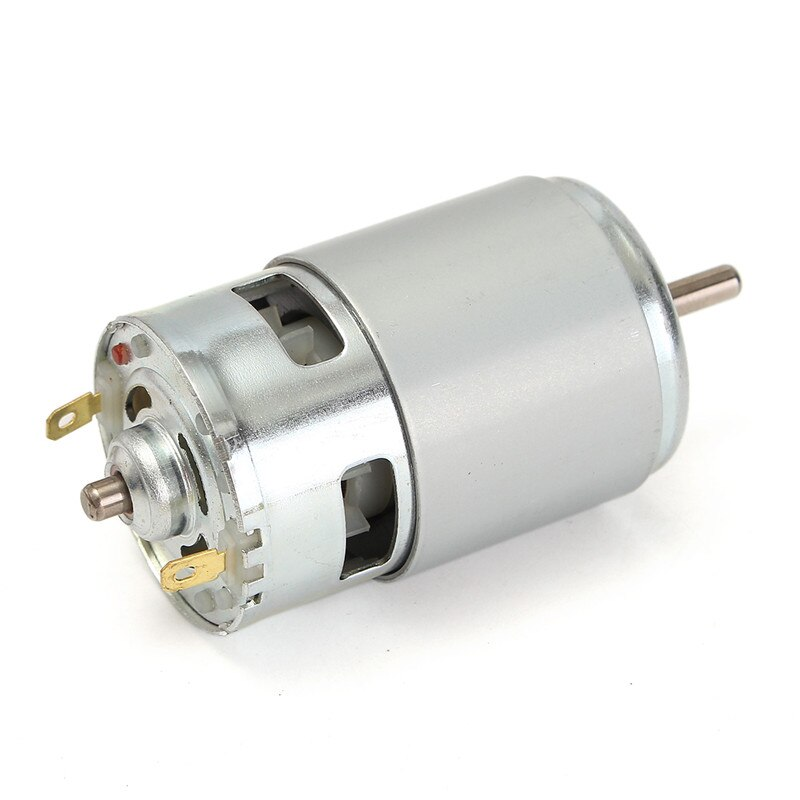
\includegraphics[width=5cm]{gambar/motorDC.jpeg}
	\caption{Jenis-Jenis \emph Joint}
\end{figure}

Motor DC dapat bergerak karena adanya elektromagnet. Saat kumparan diberi arus listrik, permukaan kumparan yang bersifat utara akan bergerak menghadap ke magnet yang berkutub selatan dan kumparan yang bersifat selatan akan bergerak menghadap ke utara magnet. Saat ini, kerena kedua kutub saling menyebabkan pergerakan kumparan berhenti. Untuk menggerakannya lagi, tepat pada saat kutub kumparan berhadapan dengan kutub magnet, arah arus pada kumparan dibalik. Dengan demikian, kutub utara kumparan akan berubah menjadi kutub selatan dan kutub selatannya akan berubah menjadi kutub utara.  

Pada saat perubahan kutub tersebut terjadi, kutub selatan kumparan akan berhadapan dengan kutub selatan magnet dan kutub utara kumparan akan berhadapan dengan kutub utara magnet. Karena kutubnya sama, maka akan terjadi tolak menolak sehingga kumparan bergerak memutar hingga utara kumparan berhadapan dengan selatan magnet dan selatan kumparan berhadapan dengan utara magnet. Siklus ini akan berulang-ulang hingga arus listrik pada kumparan diputuskan. Prinsip kerja motor DC dijelaskan pada Gambar 2.11.  

\section{Regulator}
Dalam suatu rangkaian elektronika dibutuhkan suatu sumber stabil dan sesuai dengan nilai yang dibutuhkan oleh komponen. Untuk memenuhi kebutuhan tersebut digunakanlah sebuah rangkaian regulator. Rangkaian regulator berfungsi untuk mengatur atau menghasilkan nilai tegangan pada nilai tertentu dari suatu tegangan masukan. Regulator dapat mempertahankan nilai tegangan yang keluar tanpa dipengaruhi besar arus yang dikeluarkannya. Regulator tegangan mempunyai banyak jenisnya, salah satunya adalah regulator switching.

Regulator switching mengatur besarnya nilai tegangan keluaran dengan mensaklar (ON/OFF) tegangan masukan dengan frekuensi berbeda – beda. Kelebihan dari regulator switching adalah mempunyai disipasi daya yang terjadi lebih kecil dibandingkan dengan regulator linear. Sedangkan kekurangan yaitu tegangan keluaranya akan berbentuk gelombang akibat adanya proses switching. Oleh karena itu, regulator jenis ini umumnya membutuhkan induktor, kapasitor , dan dioda untuk memperhalus tegangan keluaran. Regulator switching ada dua jenis yaitu regulator Buck dan regulator Boost. Regulator Buck untuk menghasilkan nilai tegangan keluaran yang lebih kecil dari tegangan masukannya. Sedangkan Regulator Boost untuk menghasilkan nilai tegangan yang lebih besar dari tegangan masukannya. Salah satu jenis dari regulator Buck adalah LM2596 . Bentuk fisik dari regulator Buck seperti yang ditunjukkan pada Gambar 3.2

SCARA merupakan singkatan dari \emph{Selective Compliant Assembly Robot Arm}. Robot ini pertama kali dibuat oleh perusahaan USA bernama Adept pada 1984 dan diklasifikasikan sebagai robot industri. Sistem penggerak robot SCARA merupakan pergerakan langsung pada lengan tanpa bantuan sistem \emph{belt} keculai pada bagian \emph wirst, sehingga membuat mekanisme gerakannya bekerja cepat, sederhana namun tetap akurat. Robot ini banyak digunakan sebagai robot \emph {aseembly part} dengan ukuran yang kecil degan kecepatan sedang. 


Robot SCARA yang digunakan pada penelitian ini menggunakan robot SCARA dengan nama Serpent-2. Robot Serpent-2 memiliki dua \textit{horizontal joint} yaitu bagian \textit{shoulder, elbow}dan \textit{wrist} yang dikendalikan oleh motor servo. Sedangkan pada bagian \textit{vertical joint} yang berfungsi sebagai naik turun dan buka tutup dari \emph wirst, dikendalikan oleh pneumatik yang dikontrol oleh \emph {valve relay}. Sehingga, gerakan yang terdapat pada robot SCARA dapat diklasifikasikan sebagai gerakan mengambil dan menempatkan objek. 


\begin{table}[H]
	\centering
	\caption{Spesifikasi Robot Serpent-2}
	\resizebox{6cm}{!}{%
		\begin{tabular}{|l|l|}
			\hline
			Main arm length      & 360 mm$$\hspace{2cm} 		\\ \hline
			Fore arm length      & 290 mm$$  				\\ \hline
			Shoulder movement    & 180 °$$  		\\ \hline
			Elbow movement       & 200 °$$   		\\ \hline
			Wrist rotation       & 360 °$$ 		\\ \hline
			Up \& down movement  & 150 mm$$   				\\ \hline
			Maximum tip velocity & 3.0 kg$$  				\\ \hline
			
			\end{tabular}%
		}
		\end{table}
		
		Pada bagian motor servo, robot serpent-2 menggunakan tiga buah sensor \emph feedback yang berguna sebagai pemberi nilai posisi pada masing-masing motor servo. Sensor \emph feedback yang digunakan pada robot SCARA ini menggunakan potensiometer yang memberikan nilai analog dan kemudian diproses oleh Arduino Mega 2560. Nilai ini, nantinya untuk memproses gerak kinematika dari robot SCARA tersebut sesuai dengan posisi yang diinginkan.



\section{Motor servo}
	Motor servo merupakan sebuah motor DC yang memiliki sistem \textit{feedback}. \textit{feedback} pada motor servo merupakan koreksi sudut motor DC terhadap sudut referensi \cite{Younkin2002}. pada robot Serpent-1 terdapat tiga buah motor DC, motor DC	 bagian wrist dan elbow merupakan motor DC yang identik.sehingga penulis hanya fokus membandingkan spesifikasi dua motor DC yaitu motor DC yang berada di bagian shoulder (\textit{main arm}) dan motor DC yang berada di bagian elbow (\textit{fore arm}). spesifikasi dua motor DC tersebut dapat dilihat pada tabel 2.2 sebagai berikut

\begin{table}[H]
	\centering
	\caption{Spesifikasi Motor DC pada robot Serpent-1}
	\resizebox{11cm}{!}{%
		\begin{tabular}{|l|l|}
			\hline
			Moments of inertia of the main arm ($J_{1}$)    							& $0.0980kgm^{2}$ 				\\ \hline
			Moments of inertia of the fore arm ($J_{2}$)    							& $0.0115 kgm^{2}$ 				\\ \hline
			Masses of the main arm	($m_{1}$)											& $1.90kg$   					\\ \hline
			Masses of the fore arm  ($m_{2}$)     										& $0.93kg$   					\\ \hline
			Motor and equivalent inertias ($J_{m}$)      								& $3.3*10^{-6}kgm^{2}$ 			\\ \hline
			Back emf constants for main arm and fore arm motor ($K_{e1}=K_{e2}$)  		& $0.047Nm/A$   				\\ \hline
			Armature resistance for main arm and fore arm motor($R_{a1}=R_{a2}$)		& $3.5\Omega$  					\\ \hline
			Armatures inductances for main and fore arm motor  ($L_{a1}=L_{a2}$) 		& $1.3mH$ 						\\ \hline
		\end{tabular}%
	}
\end{table}

	